\documentclass{article}

\usepackage{amsmath,amssymb,amsfonts,latexsym, amsthm}
\usepackage[spanish,es-noquoting]{babel}
\usepackage[utf8]{inputenc}
\usepackage{xcolor}
\usepackage{empheq}
\usepackage[margin=2cm]{geometry}
\usepackage[affil-it]{authblk}

\newcommand*\widefbox[1]{\fbox{\hspace{2em}#1\hspace{2em}}}
\usepackage{graphicx}
\usepackage{units}
\newtheorem{prop}{Proposición}[section]
\newtheorem{defi}{Definición}[section]
\usepackage{breqn}
\usepackage{mathptmx}
\setlength{\parindent}{0pt}
\renewcommand{\figurename}{Figure}
\begin{document}
	
	\title{Potencial Gravitacional de Yukawa en Gravedad $f(R)$}
	\author{Julián Jiménez Cárdenas\thanks{juojimenezca@unal.edu.co}}
	\affil{Universidad Nacional de Colombia.}
	\date{}
	
	\maketitle
	
	\section{Introducción}

Un acercamiento alternativo a la energía oscura es la modificación de la ley de Newton. Tal modificación surge en el límite de campo débil de algunos modelos de gravedad modificada que intentan explicar la materia oscura y la energía oscura como efectos de la curvatura del espacio tiempo. Así, en el límite de campo débil, una modificación de tipo Yukawa de la ley de Newton emerge. Uno de estos modelos es la gravedad-$f(R)$, donde la acción de Hilbert-Einstein, que es lineal respecto al escalar de Ricci $R$, se reemplaza por una función más general de la curvatura, $f(R)$. En el límite de campo débil, el potencial modificado de Newton toma la forma

\begin{equation}\label{yukawaPotential}
\Phi(r)=-\frac{GM}{(1+\delta)r}(1+\delta e^{-r(\lambda)}).
\end{equation}

Donde $M$ es la masa de la fuente puntual, $r$ es la distancia de la partícula de prueba a la fuente, $\delta$ es la fuerza de la corrección de Yukawa y $\lambda$ es la escala a la cual la fuerza de Yukawa actúa (generalmente se identifica esta escala con la longitud de onda del gravitón masivo). Hay una relación entre los parámetros de Yukawa y el Lagrangiano-$f(R)$:

\begin{equation}
	\delta=f_0'-1, \lambda=\sqrt{\frac{-6f_0''}{f_0'}},
\end{equation} 
donde $f_0'=\frac{df(R)}{dR}\Big|_{R=R_0}$ y $f_0'=\frac{d^2f(R)}{dR^2}\Big|_{R=R_0}.$

\section{Acercamiento Newtoniano al problema de dos cuerpos en el potencial de Yukawa}
En coordenadas polares, $(r,\varphi)$, y con respecto al centro de masa, las ecuaciones del movimiento son
\begin{equation}
\ddot{r}-r\dot{\varphi}^2 = -\nabla \Phi(r),
\end{equation}
\begin{equation}\label{angularConservation}
	\frac{d}{dt}(r^2\dot{\varphi})=0.
\end{equation}

La energía total del sistema se puede escribir como
\begin{equation}
	E_T=\frac{1}{2}\mu(\dot{r}^2+r^2\dot{\varphi}^2)-\frac{GMm}{(1+\delta)r}(1+\delta e^{-r/\lambda}),
\end{equation}

donde $\mu=\frac{Mm}{M+m}$ es la masa reducida. Usando la conservación del momento angular expresada en \eqref{angularConservation}, la energía se puede reescribir de la siguiente manera:

\begin{equation}
	E_T=\frac{1}{2}\mu\dot{r}^2+\underbrace{\frac{L^2}{2\mu r^2}-\frac{GMm}{(1+\delta)}\frac{(1+\delta e^{-r/\lambda})}{r}}_{V_eff(r)}.
\end{equation}

Se define el potencial efectivo como los términos de la energía total que dependen explícitamente de la posición,

\begin{equation}\label{EffPotential}
\boxed{V_{eff}:=\frac{L^2}{2\mu r^2}-\frac{GMm}{(1+\delta)}\frac{(1+\delta e^{-r/\lambda})}{r}.}
\end{equation}

Algunas consideraciones del potencial efectivo son las siguientes:

\begin{itemize}
	\item $\delta\neq -1$, para evitar que el potencial se encuentre indeterminado.
	\item Si $\delta$ toma valores negativos, el segundo término del potencial efectivo permanece atractivo siempre y cuando $\delta > -1$, y el último término se vuelve repulsivo.
	\item La condición $\delta <-1$ hace el segundo término repulsivo, y el tercer término atractivo.
	\item Si $\delta >0$, tanto el segundo como el tercer término son atractivos.
\end{itemize}

\begin{figure}
	\centering
	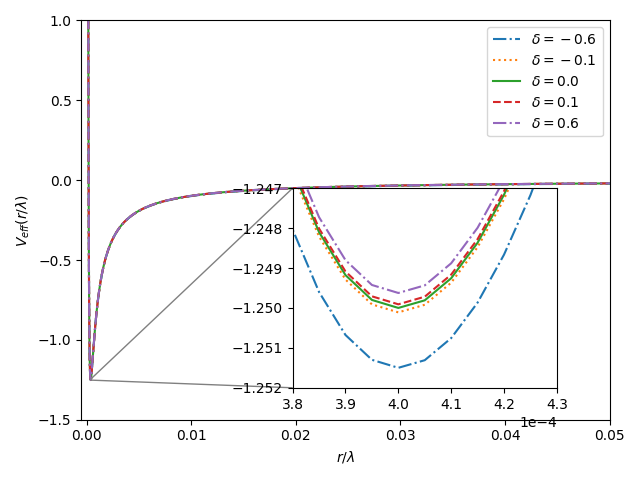
\includegraphics[width=.7\textwidth]{../veff.png}
	\caption{Potencial efectivo en función del cociente $r/\lambda$.}
	\label{fig:effPotential}
\end{figure}

\begin{figure}
	\centering
	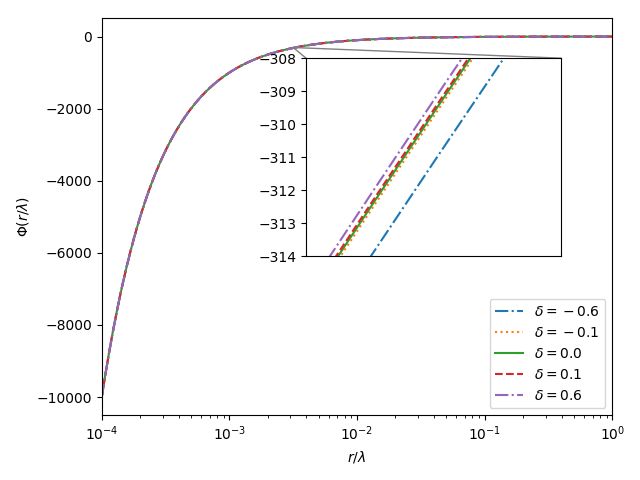
\includegraphics[width=.7\textwidth]{../potential.png}
	\caption{Potencial  en función del cociente $r/\lambda$.}
	\label{fig:potential}
\end{figure}

En las figuras \ref{fig:effPotential} y \ref{fig:potential} se muestra el comportamiento del potencial efectivo y del potencial de Yukawa en función de $r/\lambda$. Se deriva el potencial efectivo respecto a la coordenada radial para determinar los puntos críticos de éste, y encontrar bajó qué condiciones estos puntos críticos son mínimos.

\begin{dmath*}
	\frac{dV_{eff}}{dr}\Big|_{r=r_{crit}}=\frac{-L^2}{\mu r_{crit}^3}+\frac{GMm}{(1+\delta)r_{crit}^2}+\frac{GMm\delta e^{-r_{crit}/\lambda}}{(1+\delta)r_{crit}^2}+\frac{GMm\delta e^{r_{crit}/\lambda}}{\lambda(1+\delta)r_{crit}}=0.
\end{dmath*}
\begin{equation}\label{criticalCondition}
	\implies \frac{L^2}{\mu r_{crit}}=\frac{GMm(\delta e^{-r_{crit}/\lambda}+1)}{(\delta+1)}+\frac{\delta GMme^{-r_{crit}/\lambda}}{\lambda(1+\delta)}r_{crit}.
\end{equation}

Derivando nuevamente el potencial efectivo, se obtiene que

\begin{equation*}
	\frac{d^2V_{eff}}{dr^2}=\frac{3L^2}{\mu r^4}-\frac{2GMm}{(1+\delta)r^3}-\frac{2GMm\delta e^{-r/\lambda}}{(1+\delta)r^3}-\frac{GMm\delta e^{-r/\lambda}}{\lambda(1+\delta)r^2}-\frac{GMm\delta e^{-r/\lambda}}{\lambda(1+\delta)r^2}-\frac{GMm\delta e^{-r/\lambda}}{\lambda^2(1+\delta)r}.
\end{equation*}

De forma más compacta,

\begin{equation}\label{secondForm}
\frac{d^2V_{eff}}{dr^2}=\frac{3L^2}{\mu r^4}- \frac{2GMm}{(1+\delta)r^3}(\delta e^{-r\lambda}+1)-\frac{2GMm\delta e^{-r/\lambda}}{\lambda(1+\delta)r^2}-\frac{GMm\delta e^{-r/\lambda}}{\lambda^2(1+\delta)r}.
\end{equation}

Ahora, resta evaluar la ecuación \eqref{secondForm} en $r=r_{crit}$, y usar la ecuación \eqref{criticalCondition} para reescribir el término del momento angular en función de $r_{crit}$. Así, se encuentra

\begin{dmath*}
	\frac{d^2V_{eff}}{dr^2}\Big|_{r=r_{crit}}=\frac{3GMm(\delta e^{-r_{crit}/\lambda}+1)}{(\delta+1)r_{crit}^3}+\frac{3\delta GMme^{-r_{crit}/\lambda}}{(\delta+1)\lambda r_{crit}^3}r_{crit}-\frac{2GMm}{(1+\delta)r_{crit}^3}(1+\delta e^{-r_{crit}/\lambda})-\frac{2GMm\delta e^{-r_{crit}/\lambda}}{\lambda (1+\delta)r_{crit}^2}-\frac{GMm\delta e^{-r_{crit}/\lambda}}{\lambda^2 (1+\delta)r_{crit}}= \frac{GMm(\delta e^{-r_{crit}/\lambda}+1)}{(\delta+1)r_{crit}^3}+\frac{GMm\delta e^{-r_{crit}/\lambda}}{(1+\delta)r_{crit}^2}-\frac{-GMm\delta e^{-r_{crit}/\lambda}}{\lambda^2(1+\delta)r_{crit}}=\frac{GMme^{-r_{crit}/\lambda}}{(\delta+1)r_{crit}^3}\Big[ \delta\Big(1+\frac{r_{crit}}{\lambda}-\frac{r_{crit}^2}{\lambda^2}\Big)+e^{r/\lambda} \Big].
\end{dmath*}

Para garantizar que este punto crítico sea un mínimo, debe ocurrir que

$$\frac{d^2V_{eff}}{dr^2}\Big|_{r=r_{crit}}>0, \text{ es decir,}$$


$$	\frac{1}{\delta+1}\Big[ \delta\Big(1+\frac{r_{crit}}{\lambda}-\frac{r_{crit}^2}{\lambda^2}\Big)+e^{r/\lambda} \Big]>0.$$

Defina la función $g(x)$, con $x=r_{crit}/\lambda$  como

\begin{equation}\label{minimumFunction}
	\boxed{g(x)\equiv\frac{\delta(1+x-x^2)+e^{x} }{\delta+1}.}
\end{equation}

Cuando se satisfaga que $g(x)>0,$ se tendrá que el punto crítico es un mínimo. Aquí ocurre una de las primeras discrepancias con la referencia \cite{Capozziello}. Capozziello propone que la ecuación que determina si el punto crítico es mínimo es (ver ecuación (12) en \cite{Capozziello})

$$g(x)\equiv\delta(1+x-x^2)+e^{x},$$

sin el cociente de \eqref{minimumFunction}. A pesar de que ambas expresiones difieren sólo por el denominador, éste provoca que los signos de ambas expresiones de $g(x)$ difieran para las mismas condiciones. Por ejemplo, en \cite{Capozziello} se justifica que en el límite $x\rightarrow\infty$, no importa el valor de  $\delta$, $g(x)$ siempre será positivo (la exponencial domina sobre el polinomio multiplicado por $\delta$). En cambio, aunque $x\rightarrow\infty$ en \eqref{minimumFunction}, el signo de ésta dependerá de si $\delta>-1$ o $\delta<-1$. Algunas condiciones en las que \eqref{minimumFunction} es mayor que cero son las siguientes\footnote{Compare las diferencias entre estas condiciones y las condiciones de \cite{Capozziello}.}:

\begin{enumerate}
	\item $\forall\delta\neq-1$ cuando $x\rightarrow 0$.
	\item $\delta>-1$ ó $\delta<-e$ cuando $x\rightarrow 1$.
	\item $\delta>-1$ cuando $x\rightarrow\infty$.
\end{enumerate}

El primer caso, que significa que $r<<\lambda$, es la configuración de un sistema astrofísico cuya dinámica ocurre a escalas mucho menores que la longitud de onda de Compton. En este caso, es válido expandir la exponencial $e^{\pm x}$ es series de Taylor:

\begin{equation}\label{taylorExp}
	e^{\pm x}\approx 1\pm x+\frac{x^2}{2}+O(x^3).
\end{equation}

Reemplazando \eqref{taylorExp} en \eqref{yukawaPotential},

$$\Phi(r)=-\frac{GM}{(1+\delta)r}\Big(1+\delta-\frac{r\delta}{\lambda}+\frac{r^2\delta}{2\lambda^2}+O\Big(\frac{r^3}{\lambda^3}\Big)\Big)=-\frac{GM}{r}+\frac{GM\delta}{\lambda(1+\delta)}+\frac{GM\delta r}{2\lambda^2(1+\delta)}+O\Big(\frac{r^3}{\lambda^3}\Big)$$
\begin{thebibliography}{9}
	\bibitem{Capozziello} S. Capozziello, M. De Laurentis, Annalen der Physik 524, 545 (2012) 
	
	\bibitem{Lee} K. Lee, F. A. Jenet, R. H. Price, N. Wex, M. Kramer Astrophys.
	
	\bibitem{Capozziello2} S. Capozziello, M. De Laurentis, Phys. Rept. 509, 167 (2011).
	J. 722, 1589-1597 (2010)
	
	\bibitem{main} I. Martino, R. Lazkoz. Analysis of the Yukawa gravitational potential in f (R) gravity I: semiclassical periastron advance.
\end{thebibliography}
\end{document}